\subsection{Controller}\label{linear}
In order to fly the drone in a controlled manner, a PID controller is implemented.
The controller takes a desired state (for example hovering at 1.5 meters) and subtracts the output of the system, to create an "error signal".
This error signal tells the drone how displaced it is based on the magnitude of the error. The job of the controller is to correct this error through PID to drive it as close to 0 as possible, achieving a stable state/flight.

A more in depth explanation of how the PID works will be presented later in the report. 

In the figure above we see the controller model. The highlighted part is the change in Z. The PID outputs a new angular speed needed, which is divided by the change in theta and phi, since if the drone is tilted at an angle there will be a change in upwards thrust. This new value is then divided with the motor thrust coefficients to determine the magnitude of the change in Z compared to the thrust the motors provide. In short, the controller takes these changes Z depend on, and mathematically determines the change needed in angular speed for each motor, in order to go towards the desired height. \cite{Ferry}

This process is very much the same for the change in phi, theta, and yaw. The depending changes affect the outcome of the angular speed, which is put into the thrust equations to determine change for each specific motor, until the drone is stable at the set values.

It's important to note that a saturation block is put right before the output of the system to set an upper limit on the output to 3500, which is the maximum angular speed possible for the motors. This ensures that the model is realistic with the real life motors.

\begin{figure}[H]
\begin{center}
   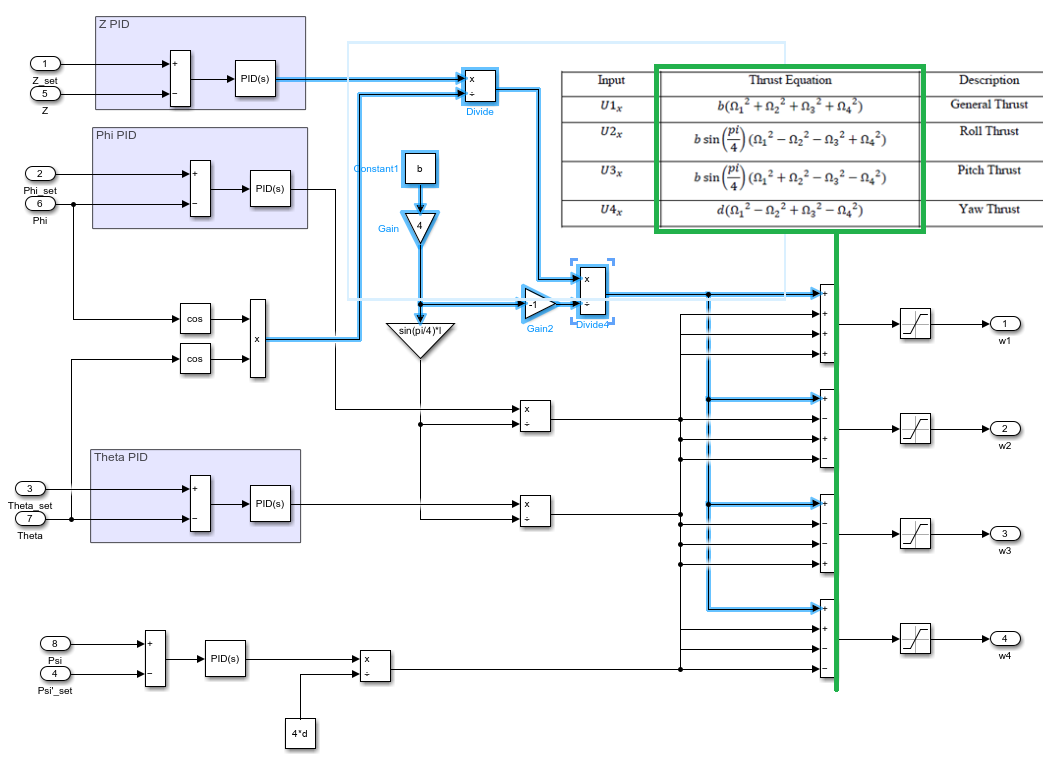
\includegraphics[scale =0.6]{pictures/control/Controller.png}
\end{center}
\caption{Overview of controller, with Z highlighted}
\end{figure}